%------------------------------------------------

\begin{fullwidth}

% Intro ----------------------------------------

% Motivation
Transforming raw data into a substantial contribution to scientific knowledge
requires a mix of subject expertise, programming skills,
and statistical and econometric knowledge.
The process of data analysis is typically
a back-and-forth discussion between people
with differing skill sets.
An essential part of the process is translating the
data originally acquired into economically meaningful indicators.
To effectively do this in a team environment,
data, code and outputs must be well-organized,
with a clear system for version control,
and analytical scripts structured such that any member of the research team can run them.
Putting in time upfront to structure the data analysis workflow
pays substantial dividends throughout the process.

% Chapter overview
In this chapter, we suggest an analytical workflow
starting from clean raw data.
We first cover variable construction:
this is when the clean data is transformed
into the actual indicators that will be used for analysis.
We emphasize the importance of transparently documenting research choices made during construction.
We then turn to analysis itself.
We do not offer instructions on how to conduct specific analyses,
as that is determined by research design;
rather, we discuss how to structure analysis code
to make sure it is easy to follow and understand.
Finally, we discuss options to automate common outputs
so that your work is fully reproducible.

\end{fullwidth}

%------------------------------------------------

\section{Constructing analysis datasets}

% What is construction
For this chapter, we assume you are starting from one or multiple tidy,\cite{hadley2017R}\sidenote{\url{Available at 
	https://vita.had.co.nz/papers/tidy-data.pdf}}
well-documented datasets that have gone through thorough quality checks,
and that incorporate any corrections needed.
No matter where you received your data from, and how well-structured it was,
in the previous chapter you can find all the steps needed to make sure it is now easy to use.
The next step is to \textbf{construct}\sidenote{\textbf{Data construction}:
The process of transforming cleaned data into analysis data by
creating the derived indicators that will be analyzed.}
the dataset, or datasets, you will use for analysis;
that is, to transform the cleaned data into analysis-ready data.
This is accomplished by integrating different datasets and creating derived variables 
(dummies, indices, and interactions, to name a few).
The derived indicator you need to construct should be
planned during research design\index{Research design},
so the pre-analysis plan can serve as a guide.\index{Pre-analysis plan}
During this process, the data will typically be 
reshaped, merged, and aggregated to change the level of the data points
from the unit of \textit{observation} in the original data 
to the unit of \textit{analysis} in the constructed data.\sidenote{\url{
		https://dimewiki.worldbank.org/Unit\_of\_Observation}}

% A project may require multiple purpose-built data sets
A constructed dataset is built to answer an analysis question.
Since different pieces of analysis may require different sub-samples,
or even different units of observation,
you may have one or many constructed datasets,
depending on your analysis plan.
You often cannot create a single ``canonical'' analysis dataset.
It is common to have many purpose-built analysis datasets.
For a concrete example of what this means,
think of an agricultural intervention that was randomized across villages
and only affected certain plots within each village.
The research team may want to run household-level regressions on income,
test for plot-level productivity gains,
and check if village characteristics are balanced.
Having three separate datasets for each of these three pieces of analysis
will result in much cleaner do-files than if they all started from 
a single analysis dataset that constantly needs to be transformed.


\begin{fullwidth}
	\begin{figure}
		\centering
		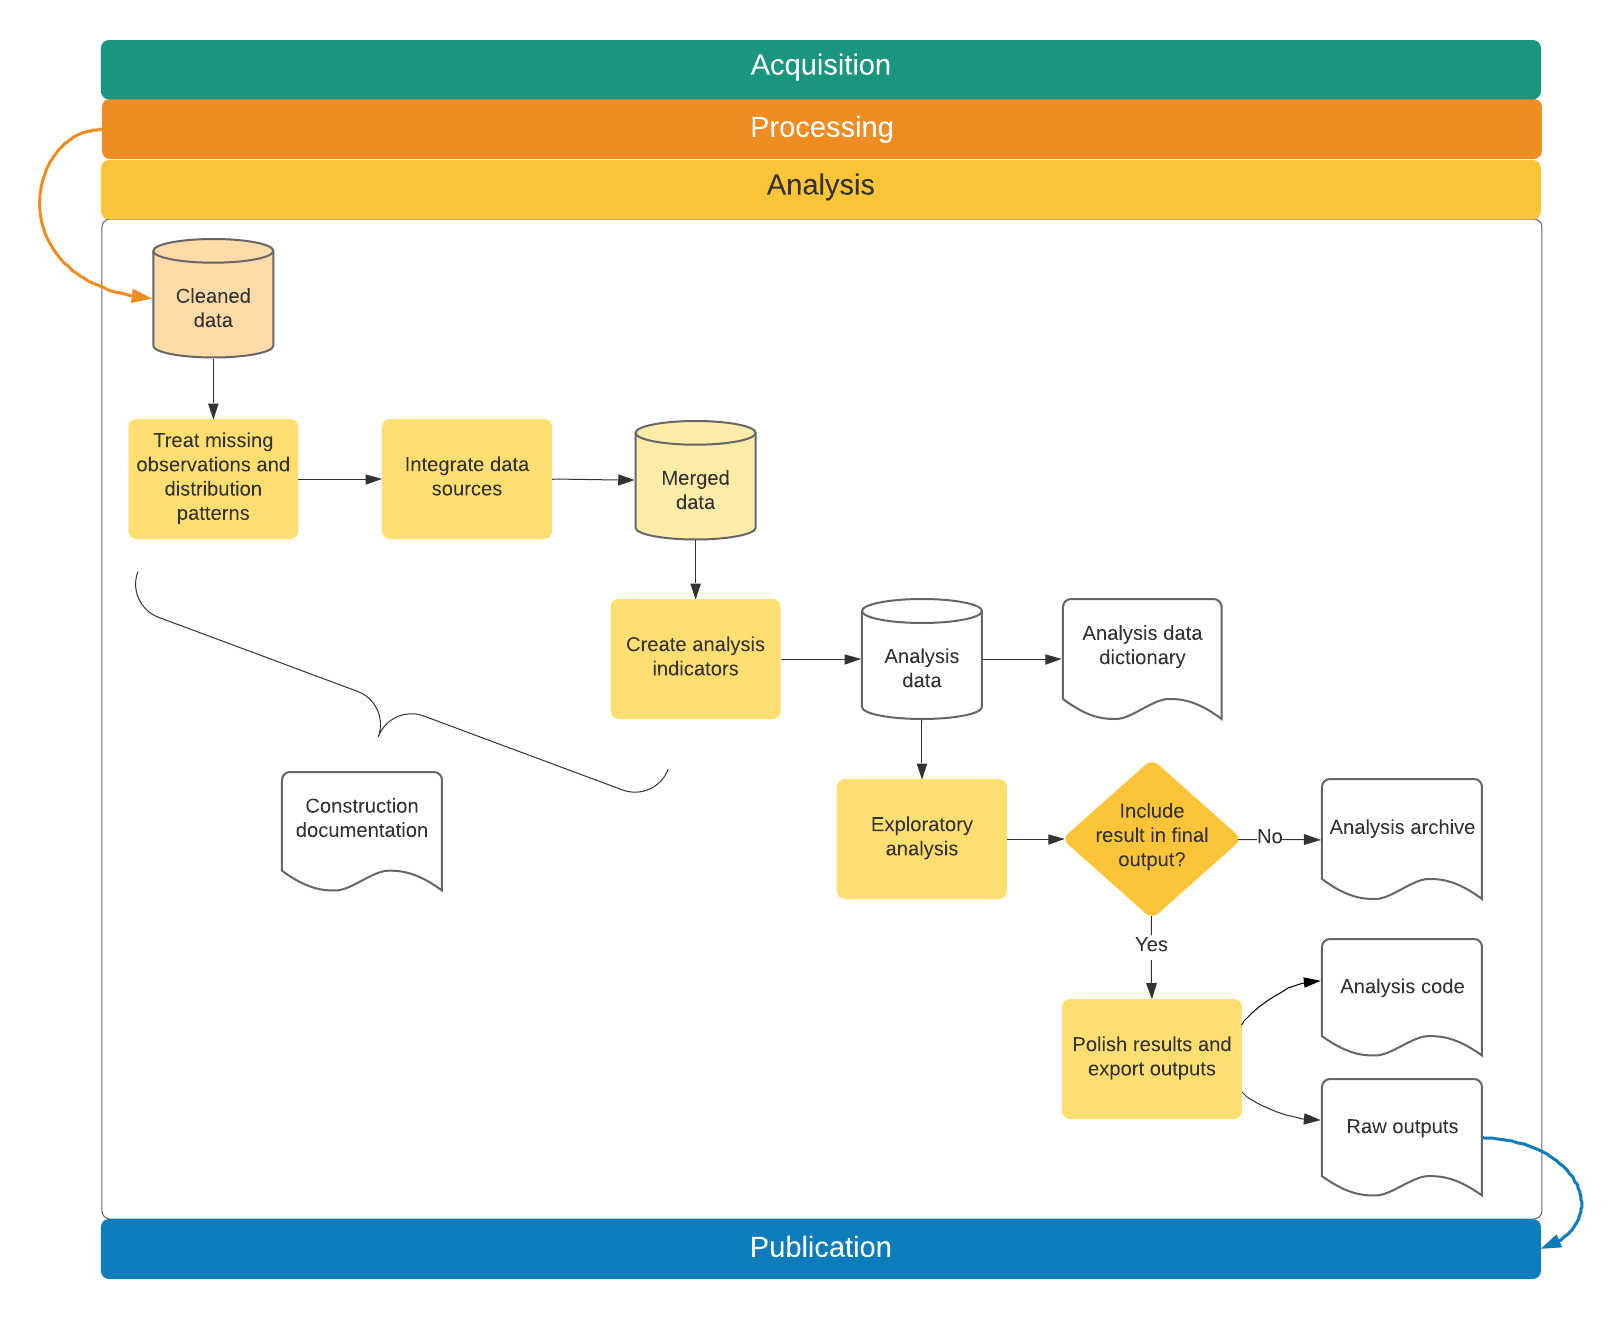
\includegraphics[width=1.6\linewidth]{diagrams/Analysis}
		\caption{}
		\label{fig:intro}
	\end{figure}
\end{fullwidth}

\subsection{Fitting construction into the data workflow}

% Why construction is separate from data cleaning
Construction is done after from data cleaning for two reasons.
First, to clearly differentiate correction of data entry errors
(necessary for all interactions with the data)
from creation of analysis indicators (necessary only for specific analyses).
Second, to ensure that variable definitions are consistent across.
Construction can create many outputs combining many inputs,
and, unlike in data cleaning, output datasets should be parsimonious rather than exhaustive.
For example, take a project that has a baseline and an endline survey.
Unless the two data collection instruments are exactly the same,
which is preferable but often not the case,
the data cleaning for each of these rounds will require different steps,
and therefore will be done separately.
However, the analysis indicators must be constructed in the exact same way, 
so they are comparable.
To do this, you will require at least two separate cleaning scripts,
and a unified construction script.
Maintaining one construction script guarantees that you will not
accidentally make changes to an indicator from one round
while forgetting to update the other.

% Why construction is separate from analysis
Construction of analysis data should be done right 
data cleaning and before data analysis,
according to the analysis plan.\index{Pre-analysis plan}
In practice, however, as you analyze the data,
different constructed variables often become necessary,
as well as different subsets of the sample
and other transformations of the data.
So you will need to adjust the analysis data accordingly.
But even if construction and analysis are done concurrently,
you should always do the two in separate scripts.
If every script that creates a table starts by loading a dataset,
subsetting it, and manipulating variables,
any edits to construction need to be replicated in all scripts.
This increases the chances that at least one of them will have a different sample or variable definition.
Doing all variable construction and data transformation
in a unified script, separate from the analysis code, helps
avoid this and ensures consistency across different outputs.

\subsection{Integrating different data sources}

% When merging is necessary and how to start thinking about it
Combining or merging information from different data sources is often times necessary
to create the analysis dataset.
For example, you may merge administrative data with survey data
to include demographic information in your analysis,
or you may want to integrate geographic information
in order to include location-specific controls.\sidenote{Such 
	operations are commonly called ``merges'' in Stata, and
	``joins'' in R's \texttt{tidyverse} dialect. 
	We will use the first term on the next few paragraphs.}
To understand how to perform such operations, 
you will need to consider the unit of observation for each dataset,
and their respective identifying variables.
Merges are common sources of missing values,
and can also result in observations being dropped.
To avoid unintentional changes to your data,
pay close attention to merge results,
and add checks to your code verifying that they match what you expect.

% Merging data sets with the same unit of observation 
If the datasets you need to merge have the same unit of observation,
merging may be straightforward.
The simplest case is when the datasets have the same unit of observation
and use a consistent, uniquely and fully identifying ID variable. 
For example, in the case of administrative data for firms,
you may merge data from different years using the firm taxpayer code
(or, preferably, a deidentified version of it).
In such cases, the main source of unexpected results are unmatched observations.
Fortunately, it is straightforward to avoid mistakes in this setting:
before writing code to combine the datasets,
write pseudocode to understand which observations you expect to be
matched or not, and why.
When possible, determine exactly which and how many 
matched and unmatched observations should result from the merge.
For example, first that were created in the second year should not be
present in the first year's data, 
and firms that closed during the first year should not be observed in the second year's data. 
Then think carefully about whether you want to keep matched and unmatched
observations, or only specific matching outcomes,
 for example, to create a balanced panel,
and add that to your pseudocode as well.
Now you can merge the datasets, 
and test that the outcome matches your expectations.
Add comments to explain any exceptions, 
and make it so the code will return an error in case unexpected results show up in future runs.
This approach can be extended to other types of merges between two related datasets.
% to-do % ----------------------------------------------------------------------------
% See XXX for an example of a Stata do-file that implements these practices -- Cami's code from TUP
% ------------------------------------------------------------------------------------

% Fuzzy matching
Even when matching data sets with the same unit of observations, however,
more complex cases may arise.
Datasets at the same unit of observation may not use a consistent identifier.
One common example is for dataset identifiers to be come in the form of names, 
which are often spelled differently in different data sources. 
In these cases, you will need to do a \textbf{fuzzy match}, 
to link observations that have similar identifiers. 
You will need to analyze the merging patterns extensively,
understand what units are present in one dataset but not the other,
and investigate unmatched observations to resolve imperfect matching.
There are some commands, such as \texttt{matchit}\sidenote{\url{
		https://ideas.repec.org/c/boc/bocode/s457992.html}} in Stata
and \texttt{agrep}\sidenote{\url{
		https://www.rdocumentation.org/packages/base/versions/3.6.2/topics/agrep}} in R,
that can provide useful utilities.
However, more often than not, a large amount of manual examination is necessary
in order to figure out what the matching pattern should be
and how to accomplish it in practice through your code.

% Merging data sets with different units of observation
Integrating datasets with different units of observation may involve changing the structure of the data.
This often involves changing the unit of observation through aggregation or reshapes.
For example, you may have data on individual students in a school,
and wish to create a summary of the student-level data set to merge to the school data, 
including variables such as gender proportions or average family income.
On the other hand, you may have asked farmers what quantity they harvested of different crops,
and need to reshape these observations to the crop level to merge with data on crop prices.
Both operations should always be done with great care. 
Two issues to pay extra attention are missing values and dropped observations.
Make sure to read about how each command treats missing observations:
are unmatched observations dropped? Are missing values turned treated as zero when aggregated?
Whenever possible, add automated checks in the script that throw an error message 
if the result is different than what you expect.
If you are subsetting your data, prefer to drop observations explicitly,
indicating why you are doing so and how the data set changed.
% to-do % -----------------------------------------------------------------
% See XXX for an example of a Stata do-file that implements these practices
% -------------------------------------------------------------------------

% Data integration
Note, however, that not all merges of data with different units of observation 
are as conceptually straightforward.
More complex cases may arise if you are looking to overlay road location data with household data,
using a spatial match;
to combine school administrative data, such as attendance records and test scores,
with household demographic characteristics from a survey;
or link a dataset of infrastructure access points, such as water pumps or schools,
and a dataset of household locations.
In these cases, a key part of the research contribution is figuring out what
a useful way to combine the datasets is.
Since the conceptual constructs that link observations from the two data sources
are so important and can take many possible forms,
it is especially important for the data integration to not be treated mechanically,
and to be extensively documented separately from other data construction tasks.


\subsection{Creating analysis variables}

% Main points to keep in mind for new variables
Once you have assembled variables from different sources into a single working dataset
with the right raw information and observations,
it's time to create the derived indicators of interest for analysis. 
Before constructing new indicators,
you must check and double-check units, scales and value assignment of each variable that will be used.
This is when you will use the knowledge of the data and the documentation developed during cleaning the most.
First, check that all categorical variables have the same value assignment, i.e.,
that labels and levels have the same correspondence across variables that use the same options.
For example, it's possible that in one question \texttt{0} means ``no'' and \texttt{1} means ``yes'',
while in another one the same answers were coded as \texttt{1} and \texttt{2}.
(We recommend coding binary questions as either \texttt{1} and \texttt{0} or \texttt{TRUE} and \texttt{FALSE},
so they can be used numerically as frequencies in means and as dummies in regressions.
Note that this implies re-expressing categorical variables like \texttt{gender} to binary variables like \texttt{woman}.)
Second, make sure that any numeric variables you are comparing are converted to the same scale or unit of measure:
you cannot add one hectare and two acres and get a meaningful number.
New variables should be assigned functional names, 
and the dataset ordered such that related variables are together.
Adding notes to each variable will make your dataset more user-friendly.

% Dealing with outliers and missing values
At this point, you will also need to decide how to handle any outliers or unusual values identified during data cleaning. 
How to treat outliers is a research question.
There are multiple possible approaches, 
and the best choice for a particular case will depend on the objectives of the analysis.
Whatever your team decides, make sure to explicitly note what the decision was and how it was made.
Results can be sensitive to the treatment of outliers,
so keeping the original variable in the dataset will allow you to test how much it affects the estimates.
All these points also apply to imputation of missing values and other distributional patterns.
As a general rule, never overwrite or delete original data during the construction process.

% Maintaining indicator definition across rounds
Finally, creating a panel with survey data involves additional timing complexities.
It is common to construct indicators soon after receiving data from a new survey round.
However, creating indicators for each round separately increases the risk of using different definitions every time.
Having a well-established definition for each constructed variable helps prevent that mistake,
but the best way to guarantee it won't happen is to create the indicators for all rounds in the same script.
Say you constructed some analysis variables after baseline, and are now receiving midline data.
Then the first thing you should do is create a cleaned panel dataset,
ignoring the previous constructed version of the baseline data.
Our team created \texttt{iefieldkit}'s \texttt{iecodebook append} subcommand
% to-do % -----------------------------------------------------------------
% \sidenote{\url{STATA JORUNAL ARTICLE}}
% -------------------------------------------------------------------------
to help you reconcile and append data from cleaned survey rounds.
This is done by filling an Excel sheet to indicate what changes in
names, value assignments and value labels should be made so the data is consistent across rounds.
By doing so, you are also creating helpful documentation about your data work.
% to-do % --------------------------------------------------------
% See XXX for an example of a Stata do-file uses iecodebook append
% ----------------------------------------------------------------
Once rounds are consistently appended, 
adapt your construction script so it can be used on the complete panel dataset.
In addition to preventing inconsistencies and documenting your work,
this process will also save you time and give you an opportunity to review your original code.


\subsection{Documenting variable construction}

% Why documentation is important: transparency and reproducibility
Because data construction involves translating concrete observed data points
to measures of abstract concepts,
it is important to document exactly how each variable is derived or calculated.
Careful documentation is closely linked to the research principles discussed in the first chapter.
It makes research decisions transparent, 
as anyone can read about how you defined each variable in your analysis,
and what was the reasoning behind these decisions.
By reading the documentation, 
someone unfamiliar with the project should be able to understand the contents of the analysis datasets,
the steps taken to create them, and the decision-making process through your documentation.
Ideally, they should also be able reproduce your steps and recreate the constructed variables.
Therefore, documentation is an output of construction as relevant as the code and data,
and it is good practice for papers to have an accompanying data appendix
listing analysis variables and their definitions.

% How to document construction
The development of construction documentation is a good opportunity to have 
a wider discussion with your team about creating protocols for variable definition,
which will guarantee that indicators are defined consistently across projects.
Whether you do that or not,
make sure to have a detailed account of how variables are created.
This will be implemented in your code, but you should still
add comments to it explaining in human language what you are doing and why.
This is a crucial step both to prevent mistakes and to guarantee transparency.
To make sure that these comments can be more easily navigated,
it is wise to start writing a variable dictionary as soon as you begin making changes to the data.
Carefully record how specific variables have been combined, recoded, and scaled,
and refer to those records in the code.

% iecodebook export
The \texttt{iecodebook export} subcommand is 
a good way to ensure you have easy-to-read documentation.
When all your final indicators have been created,
you can use the it to list all variables in the dataset in an Excel sheet.
You can then add the variable definitions to that file to create a concise metadata document.
Take this opportunity to review your notes and make sure that your code
is implementing exactly what is described in the documentation.
% to-do % --------------------------------------------------------
% See XXX for an example of a Stata do-file uses iecodebook append
% ----------------------------------------------------------------

%------------------------------------------------

\section{Writing data analysis code}

% Intro: this section focuses on data analysis CODE
After data is cleaned and indicators are constructed, you are ready to generate analytical outputs.
\index{data analysis}
There are many existing resources for data analysis and statistical methods, such as
\textit{R for Data Science};\cite{hadley2017R}\sidenote{Available at \url{https://r4ds.had.co.nz}}
\textit{A Practical Introduction to Stata};\cite{RePEc:gdm:wpaper:9412}\sidenote{Available at \url{https://scholar.harvard.edu/files/mcgovern/files/practical_introduction_to_stata.pdf}}
\textit{Mostly Harmless Econometrics};\cite{angrist2008mostly}
and \textit{Causal Inference: The Mixtape}.\sidenote{\url{https://scunning.com/mixtape.html}}
We focus on how to structure analytical code and files, rather than how to conduct specific analyses.

\subsection{Organizing analytical code}

% Exploratory vs final data analysis 
The analysis stage usually starts with a process we call \textbf{exploratory data analysis}.
This is when you are first looking for patterns in your data,
creating descriptive graphs and tables,
and trying different tests to understand your results.
It progresses into \textbf{final analysis} when your team starts to decide which are the ``main results'', or
those that will make it into a research output.
The way you deal with code and outputs for exploratory and final analysis is different.
During exploratory data analysis,
you will be tempted to write lots of analysis into one big, impressive, start-to-finish script.
While this is fine when you are writing your research stream of consciousness into code, 
it leads to poor practices in the final code such as not clearing the workspace 
and not loading a fresh constructed dataset before each analysis task.

% Write independent analysis scripts
To avoid mistakes, it's important to take the time
to organize the code that you want to keep, that is,
the final analysis code, in a clean manner.
The result is a curated set of polished scripts that will be part of a reproducibility package.
A well-organized analysis script starts with a completely fresh workspace
and, for each output it creates, explicitly loads data before analyzing it.
This setup encourages data manipulation to be done earlier in the workflow
(that is, in separate cleaning and construction scripts).
It also prevents you from accidentally writing pieces of analysis code that depend on one another
or that require manual instructions for all necessary chunks of code to be run in the right order.
IT also encourages you to rewrite each task so it is completely independent of all other code,
except for the master script.
You could go as far as coding every output in a separate script.

% Writing easy to read analysis code
There is nothing wrong with code files being short and simple.
In fact, analysis scripts should be as simple as possible,
so whoever is reading them can focus on the concepts, not the coding.
Research questions and statistical decisions should be incorporated explicitly in the code through comments,
and their implementation should be easy to detect from the way the code is written.
This includes clustering, sampling, and controlling for different variables, to name a few.
If you have multiple analysis datasets,
each of them should have a descriptive name about its sample and unit of observation.
As your team comes to a decision about model specification,
you can create functions and globals (or objects) in the master script to use across scripts.
This is a good way to make sure specifications are consistent throughout the analysis.
It also makes your code more dynamic,
as it's easy to update specifications and results 
through a master file without changing every script.

% to-do % ------------------------------------------------------------------------
% Add example of how to automatize research decisions through globals or functions
% --------------------------------------------------------------------------------

% Naming analysis code
To accomplish this, you will need to make sure that you have an effective data management system,
including naming, file organization, and version control.
Just like you did with each of the analysis datasets,
name each of the individual analysis files descriptively.
Code files such as \path{spatial-diff-in-diff.do},
\path{matching-villages.R}, and \path{summary-statistics.py}
are clear indicators of what each file is doing, and allow you to find code quickly.
If you intend to numerically order the script files 
to correspond to exhibits as they appear in a paper or report,
leave this to near publication time.

\subsection{Visualizing data}

% Useful resources for data visualization
\textbf{Data visualization}\sidenote{\url{
		https://dimewiki.worldbank.org/Data\_visualization}} \index{data visualization}
is increasingly popular, 
and is becoming a field in its own right.\cite{healy2018data,wilke2019fundamentals}
Whole books have been written on how to create good data visualizations,
so we will not attempt to give you advice on it.
Rather, here are a few resources we have found useful.
The Tapestry conference focuses on ``storytelling with data''.\sidenote{
	\url{https://www.youtube.com/playlist?list=PLb0GkPPcZCVE9EAm9qhlg5eXMgLrrfMRq}}
\textit{Fundamentals of Data Visualization} provides extensive details on practical application;\sidenote{
	\url{https://serialmentor.com/dataviz}}
as does \textit{Data Visualization: A Practical Introduction}.\sidenote{
	\url{http://socvis.co}}
Graphics tools in Stata are highly customizable.
There is a fair amount of learning curve associated with extremely-fine-grained adjustment,
but it is well worth reviewing the graphics manual.\sidenote{\url{
		https://www.stata.com/manuals/g.pdf}}
For an easier way around it, Gray Kimbrough's 
\textit{Uncluttered Stata Graphs}
code is an excellent default replacement for Stata graphics that is easy to install.\sidenote{
	\url{https://graykimbrough.github.io/uncluttered-stata-graphs}}
If you are an R user, the \textit{R Graphics Cookbook}\sidenote{\url{
		https://r-graphics.org}}
is a great resource for the its popular visualization package \texttt{ggplot}\sidenote{
	\url{https://ggplot2.tidyverse.org}}.
But there are a variety of other visualization packages,
such as \texttt{highcharter},\sidenote{\url{http://jkunst.com/highcharter}}
\texttt{r2d3},\sidenote{\url{https://rstudio.github.io/r2d3}}
\texttt{leaflet},\sidenote{\url{https://rstudio.github.io/leaflet}}
and \texttt{plotly},\sidenote{\url{https://plot.ly/r}} to name a few.
We have no intention of creating an exhaustive list, 
but these are good places to start.

% Writing data viz code
We attribute some of the difficulty of creating good data visualization
to writing code to create them.
Making a visually compelling graph would already be hard enough if
you didn't have to go through many rounds of googling to understand a command.
The trickiest part of using plotting commands is getting the data into the right format.
Though both Stata and R have plotting functions that graph summaries of the data,
a good rule of thumb that you can be sure will always work is for each
observations in your data set to correspond to one data point your want 
to represent in your plot.
This may seem simple, 
but may require you to do some of the aggregation and reshaping operations
discussed earlier in this chapter.

% Stata Visual Library and ietoolkit
Based on DIME's accumulated experience creating visualizations for impact evaluations, 
our team has developed a few resources to facilitate this workflow.
First of all, we maintain a \textbf{Stata Visual Library}\sidenote{
	\url{https://worldbank.github.io/Stata-IE-Visual-Library}},
which has examples of graphs created in Stata and curated by us.\sidenote{
	A similar resource for R is \textit{The R Graph Gallery}. 
	\\ \url{https://www.r-graph-gallery.com}}
The Stata Visual Library includes example datasets to use with each do-file,
so you get a good sense of what your data should look like
before you can start writing code to create a visualization.
The \texttt{ietoolkit} package also contains two commands to automate
common impact evaluation graphs: 
\texttt{iegraph} plots the values of coefficients for treatment dummies,
and \texttt{iekdensity} displays the distribution of an outcome variable
across groups and adds the treatment effect as a note.


%-------------------------------------------------------------------------
\section{Creating analysis outputs}

% Intro: why to think about outputs ahead of time
A great number of outputs will be created during the course of a project.
These will include both raw outputs such as tables and graphs
and final products such as presentations, papers and reports.
During exploratory analysis, your team will consider different approaches
to answer research questions and present answers.
Though it is best to be transparent about different
specifications tried and tests performed,
only a few will be considered ``main results''.
When the first outputs are being created, agree on where to store them,
what software and formats to use, and how to keep track of them.
This discussion will save you time and efforts on two fronts:
formatting and polishing tables and graphs that 
will not make their way into final research products;
and remembering the different paths your team has already
taken, so you don't do the same thing twice.
This section will take you through key elements to keep in mind 
when making workflow decisions and outputting results.


\subsection{Managing outputs}

% Where to store outputs
Decisions about storage of outputs are made easier by technical constraints.
As discussed above, version control systems like Git are a great way to manage
plain text files, and sync software such as Dropbox and OneDrive are better for binary files.
Outputs will similarly come in these two formats, depending on your software.
Binary outputs like Excel files, PDFs, PowerPoints, or Word documents can be kept in a synced folder.
Raw outputs in plain text formats like \texttt{.tex} and \texttt{.csv}
can be created from most analytical software and managed with Git.
Tracking plain text outputs with Git facilitate the identification of changes in results.
If you are re-running all of your code from the master script,
the outputs will be overwritten,
and any changes in coefficients and number of observations, for example, so
will be automatically flagged for you or a reviewer to check.
Tracking changes to binary files such as images is a bit more cumbersome, as they use more space.
This may cause your syncing to the cloud to be slower.
But it is still a good way to know when changes in the code affect outputs,
depending on the git client you are using.
GitHub desktop, for example, displays changes in images files in an accessible manner.

% Tracking scripts and their outputs
Independently of your storage decisions,
you will need to update your outputs frequently.
And if you have tried to recreate a result after a few months,
you probably know that it can be hard to remember where the code that created it was saved.
Naming conventions and code organization,
including easily searchable file names and comments,
play a key role in not re-writing scripts again and again.
It is common for teams to maintain one ``final'' analysis file
and one folder with draft code or exploratory analysis.
The latter contains pieces of code that are stored for reference,
but not cleaned up to be included in any final outputs.
Once an output presents a result in the clearest manner possible,
it should be renamed and moved to the ``final analysis'' folder.
It's typically desirable to have the names of outputs and scripts linked --
so, for example, \texttt{factor-analysis.do} creates \texttt{factor-analysis.eps} and so on.
Document output creation in the master script that runs your code,
so that before the line that runs a particular analysis script
there are a few lines of comments listing
datasets and functions that are necessary for it to run,
as well as all outputs created by that script.

% to-do % ----------------------
% Add an example analysis master
% ------------------------------

% File formats
Agree with your team on what tools will be used for what outputs, 
and where they will be stored, before you start creating them.
Take into account ease of use for different team members, and
keep in mind that learning how to use a new tool may require some
time investment upfront that will be paid off as your project advances.
Knowing how your code outputs will be used will help you decide the best format to export them.
You can typically use the same command to save figures into different formats, 
such as \texttt{.eps}, \texttt{.png}, \texttt{.pdf} or \texttt{.jpg}.
However, the decision between using Office Suite software such as Word and Power Point
versus {\LaTeX} and other plain text formats may influence how you write your code,
as this choice often implicates in the use of a particular command.
We strongly recommend that you chose software to create final products
that can be linked to raw outputs in such a way that they are updated
in the paper or presentation every time changes are made to them.
We broadly call files that have this feature \textbf{dynamic documents},
and they will be discussed in more detail in the final section of this chapter.


\subsection{Exporting analysis outputs}

% Which outputs should be fully automated and why
As briefly discussed in the previous section,
you do not \textit{need} to export each and every table and graph created during exploratory analysis.
Most statistical software allow you to review results interactively,
and this is often preferred at this stage.
Final analysis scripts, on the other hand, must export outputs
that are ready to be included in a paper or report.
No manual edits, including formatting, 
should be necessary after exporting final outputs.
Manual edits are difficult to replicate.
You may think that it's not worth coding a small formatting adjustment,
but you will inevitably need to make changes to the output,
and automating them will save you time by the end of the process.
On the other hand, don't spend much time formatting tables and graphs until 
you have come to a decision about which will be used for your final product.\sidenote{
	For a more detailed discussion on this, including different ways to export tables from Stata, see \url{https://github.com/bbdaniels/stata-tables}}
Polishing final outputs can be a time-consuming process,
and you want to do it as few times as possible.

% Don't copy-paste!!
We cannot stress this enough:
do not set up a workflow that requires copying and pasting results.
Copying results from Excel to Word is error-prone and inefficient.
Copying results from a software console is risk-prone,
even more inefficient, and totally unnecessary.
The amount of work needed in a copy-paste workflow increases
rapidly with the number of tables and figures included in a research output,
and so do the chances of having the wrong version of a result in a paper or report.

% Output formats
There are numerous commands to export outputs from both R and Stata to a myriad of formats.
Some examples are \texttt{estout},\cite{estout05, estout07}\sidenote{Documentation available at \url{http://repec.sowi.unibe.ch/stata/estout/}.}
\texttt{outreg2},\sidenote{\url{https://www.princeton.edu/~otorres/Outreg2.pdf}}
and \texttt{outwrite}\sidenote{\url{https://www.benjaminbdaniels.com/stata-code/outwrite}} in Stata,
and \texttt{stargazer}\sidenote{\url{https://cran.r-project.org/web/packages/stargazer/vignettes/stargazer.pdf}}
and \texttt{ggsave}\sidenote{\url{https://ggplot2.tidyverse.org/reference/ggsave.html}} in R.
Save outputs in accessible and, whenever possible, lightweight formats.
Accessible means that it's easy for other people to open them.
In Stata, that would mean always using \texttt{graph export} to save images as
\texttt{.jpg}, \texttt{.png}, \texttt{.pdf}, etc.,
instead of \texttt{graph save},
which creates a \texttt{.gph} file that can only be opened by Stata.
Some publications require ``lossless'' TIFF or EPS files, 
which are created by specifying the desired extension.
Whichever format you decide to use, 
remember to always specify the file extension explicitly.
For tables, there are fewer.
Given our recommendation to use \textbf{dynamic documents},
which will be discussed in more detail both in the next section and in chapter \ref{ch:7},
exporting tables to \texttt{.tex} is preferred.
Excel \texttt{.xlsx} and \texttt{.csv} are also commonly used,
but require the extra step of copying the tables into the final output.
The \texttt{ietoolkit} package includes two commands to export formatted tables,
automating the creation of common outputs and saving time for research.
\texttt{iebaltab}\sidenote{\url{https://dimewiki.worldbank.org/iebaltab}}
creates and exports balance tables to Excel or {\LaTeX}.
\texttt{ieddtab}\sidenote{\url{https://dimewiki.worldbank.org/ieddtab}}
does the same for difference-in-differences regressions.

% Last touches: formatting tables and including meta data
If you need to create a table with a very specific format
that is not automated by any command you know, consider writing it manually
(Stata's \texttt{filewrite} and R's \texttt{cat()}, for example, allow you to do that).
This will allow you to write a cleaner script that focuses on the econometrics,
and not on complicated commands to create and append intermediate matrices.
Keep in mind that final outputs should be self-standing.
This means it should be easy to read and understand them with only the information they contain.
Make sure labels and notes cover all relevant information 
included in your code and comments that are not otherwise visible in the output.
Examples of this include sample, 
unit of observation, unit of measurement, and variable definition.\sidenote{
	\url{https://dimewiki.worldbank.org/Checklist:\_Reviewing\_Graphs} and
	\url{https://dimewiki.worldbank.org/Checklist:\_Submit\_Table}}
It is usually preferable to add labels and notes to tables and figures 
directly in the documents, rather than through code.
This will make their formatting more consistent.

\section{Preparing dynamic documents}

% Intro: what it is and why to use it
Dynamic documents are a broad class of tools that enable a streamlined, reproducible workflow.
The term ``dynamic'' can refer to any document-creation technology
that allows the inclusion of explicitly encoded linkages to raw output files.
This means that, whenever outputs are updated,
the next time the document is loaded or compiled, it will automatically include
all changes made to all outputs without any additional intervention from the user.
This is not possible in tools like Microsoft Office,
although there are tools and add-ons that produce similar functionality.
In Word, by default, you have to copy and paste each object individually
whenever tables, graphs, or other inputs have to be updated.
This workflow becomes more complex as the number of inputs grows,
increasing the likelihood of making mistakes or missing updates.
Dynamic documents prevent this from happening by managing document compilation and
inclusion of inputs in a single integrated process,
so you can skip the copying and pasting altogether.
Alternatively, if your team prefers to use static documents they are already familiar with,
prefer not compiling outputs into a document at all, at least in exploratory work.

\subsection{Dynamic exploratory analysis}	

% Markdown
If all team members working on a dynamic document are comfortable using the same statistical software,
built-in dynamic document engines are also a good option.
This means you can write both text (often in Markdown\sidenote{\url{https://www.markdownguide.org/}}) and code in the script,
and the result will usually be a PDF or HTML file including code, text, and outputs.
In our experience, however, many researchers find the entry cost to learning how to use these tools too high.
These types of dynamic document tools are typically best used by the team members that work more closely with code,
and can be great for creating exploratory analysis reports as you work on them, 
or paper appendices including large chunks of code and dynamically created graphs and tables.
RMarkdown\sidenote{\url{https://rmarkdown.rstudio.com}} is the most widely adopted solution in R.
Stata offers a built-in package for dynamic documents, \texttt{dyndoc}\sidenote{\url{
		https://www.stata.com/manuals/rptdyndoc.pdf}}, 
and user-written commands such as \texttt{markstat},\sidenote{\url{https://data.princeton.edu/stata/markdown}}
\texttt{webdoc},\sidenote{\url{http://repec.sowi.unibe.ch/stata/webdoc}} and
\texttt{texdoc}.\sidenote{\url{http://repec.sowi.unibe.ch/stata/texdoc}}
The great advantage of these tools in comparison with LaTeX is that 
they create full documents from within your scripts, 
so running the code and compiling the document is reduced to a single step.

% Non-code options
Documents called ``notebooks'' (such as Jupyter\sidenote{\url{https://jupyter.org}}) work similarly,
as they also use the underlying analytical software to create the document.
These tools are usually appropriate for short or informal documents
because it tends to be difficult for those who are not familiar with them to edit the content,
and they often don't offer as extensive formatting options as, for example, Word.
There are also simple tools for dynamic documents
that do not require direct operation of the underlying code or software,
simply access to the updated outputs.
An example of this is Dropbox Paper,
a free online writing tool that can be linked to files in Dropbox
which are automatically updated anytime the file is replaced.
They have limited functionality in terms of version control and formatting,
and may never include any references to confidential data,
but they do offer extensive collaboration features, 
and can be useful for working on informal outputs. 
Markdown files on GitHub can also provide similar functionality through the browser,
and are version controlled.
However, as with other Markdown options, the need to learn a new syntax may
discourage take up among team members who don't work with GitHub more extensively.

\subsection{Dynamic research outputs: the case for {\LaTeX}}

% What is LaTeX
Though formatted text software such as Word and PowerPoint are still prevalent,
researchers are increasingly choosing to prepare final outputs
like documents and presentations using {\LaTeX}.\index{{\LaTeX}},\sidenote{See
	\url{https://www.latex-project.org} and \url{https://github.com/worldbank/DIME-LaTeX-Templates}.}
{\LaTeX} is a document preparation and typesetting system with a unique code syntax.
While this tool has a significant learning curve,
its enormous flexibility in terms of operation, collaboration, output formatting, and styling
make it our preferred choice for most large technical outputs.
In fact, {\LaTeX} operates behind-the-scenes in many other dynamic document tools (discussed below).
Therefore, we recommend that you learn {\LaTeX} as soon as you are able to.

% Advantages of LaTeX
The main advantage of using {\LaTeX} is that it updates outputs every time the document is compiled,
while still allowing for text to be added with a relative simple syntax and user-friendly interface.
Additionally, because of its popularity in the academic community,
social scientists are more familiar with it than other dynamic documents tools,
so the cost of entry for a team is often relatively lower.
Because \texttt{.tex} files are plain text, 
they can be version-controlled using Git.
Creating documents in {\LaTeX} using an integrated writing environment such as TeXstudio, TeXmaker or LyX
is great for outputs that focus mainly on text
and include figures and tables that may be updated.
It is good for adding small chunks of code into an output.
This book, for example, was written in {\LaTeX} and managed on GitHub.\sidenote{\url{
		https://github.com/worldbank/d4di}}
Finally, some journals make {\LaTeX} templates available,
so papers can be more easily be formatted into their specific layout. 
	

%------------------------------------------------
